\subsection{Dolní propust 2. řádu}\label{s:DP2}
Dolní propust druhého řádu má přenos v nekonečnu nulový $H_{\infty} = 0$. Přenosová funkce je
\begin{align}
H(j\omega) = \frac{H_0 \omega_c ^2}{(j\omega)^2 + \frac{\omega _c}{Q}(j\omega) + \omega _c ^2}.
\end{align}
\noindent Obvodová simulace byla realizována v programu Multisim. Bylo zvoleno symetrické napájení OZ $V_{DD},V_{SS} = \pm 15$ V. Regulací vstupního proudu je ovlivňován pracovní bod obvodu (mezní kmitočet). Vstupní externí proud $I_{ABC} = 0.5$ $\mu$A byl zvolen tak, aby byl obdržen mezní kmitočet cca 100 kHz. Externím proudem $I_{ABC} \in$ $[5$ $\mu$A ; 500 $\mu$A] je garantováno minimální výstupní napětí $U_{OUT} = \pm 12$ V, standardně $V_{peak 1} = 14.2$ V a $V_{peak 2} = -14.4$ V. Při výstupním napětí v tomto intervalu je šum vzhledem k signálu zanedbatelný a nezkreslí výsledky simulace.\\
\noindent Bylo použito zapojení s paralelně řazeným uzemněným kapacitorem a odporem a indukčností. Na výstupu 2. OTA (V1) byl obdržen filtr typu PP 1. řádu. Na výstupu 3. OTA (V2) pak DP 2. řádu.
\begin{figure}[h]
\centering
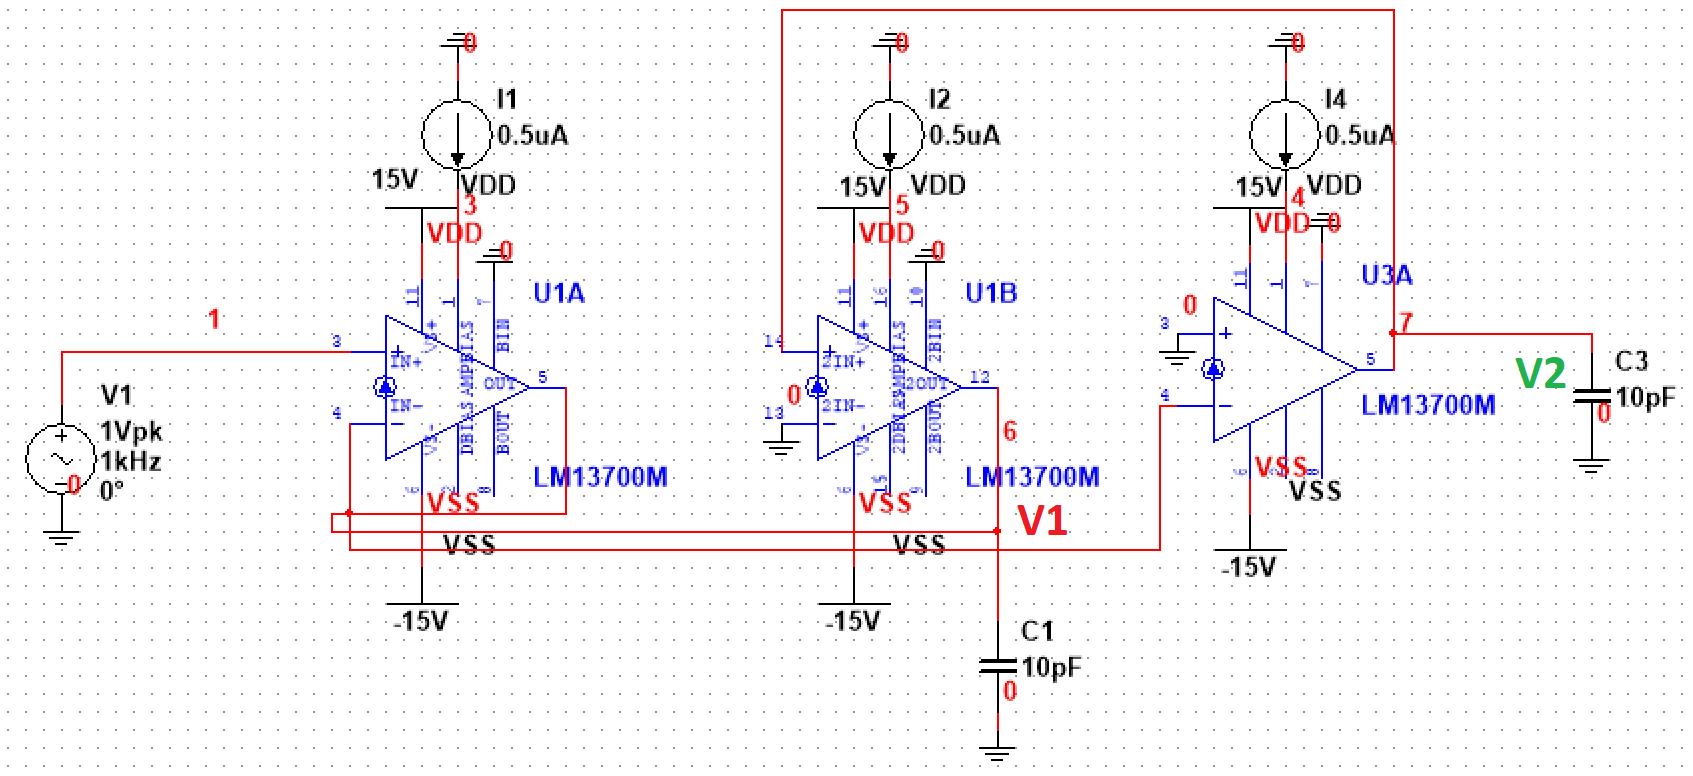
\includegraphics[scale=0.3]{bplp.png}
\caption{Schéma zapojení DP 2. řádu}
\end{figure}\begin{figure}[h]
\centering
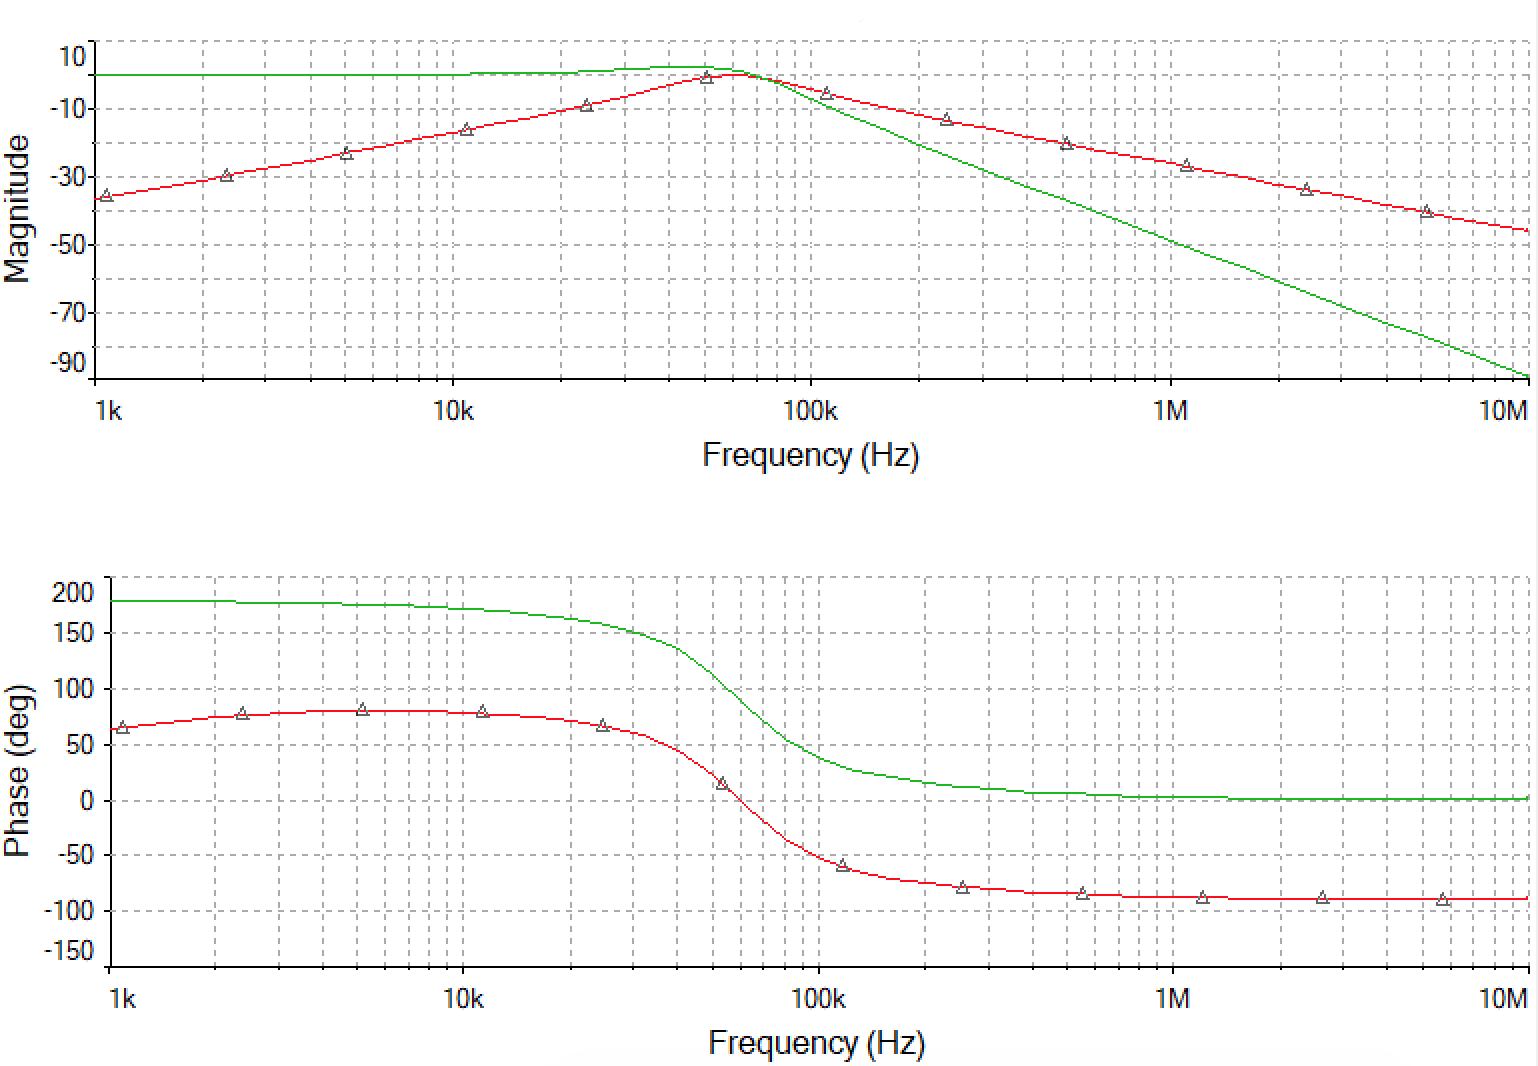
\includegraphics[scale=0.5]{bplp2.png}
\caption{Amplitudová a fázová charakteristika DP 2. řádu, PP}
\end{figure}
\subsection{Dolní propust 4. řádu}\label{s:DP4}
Kaskádní zapojení sestává ze sériově zapojených bloků.
\begin{figure}[h]
\centering
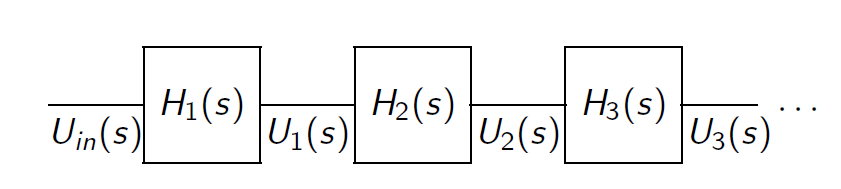
\includegraphics[scale=0.4]{schemata.png}
\caption{Kaskádní zapojení \cite{5}}
\end{figure}
\noindent Přenosové funkce jednotlivých bloků se násobí
\begin{align}
H_k(j\omega) = \frac{U_k (j\omega)}{U_{k-1}(j\omega)}.
\end{align}
Přenos posledního bloku je dán vztahem
\begin{align}
H_{1 \rightarrow k}(j\omega) = \frac{U_k (j\omega)}{U_{in}(j\omega)} = \prod _{n=1}^{k} H_n(j\omega).
\end{align}
Kaskádním zapojením dvou dolních propusti ze sekce \ref{s:DP2} byl obdržen filtr 4. řádu s poklesem -80 dB/dek.
\begin{figure}[h]
\centering
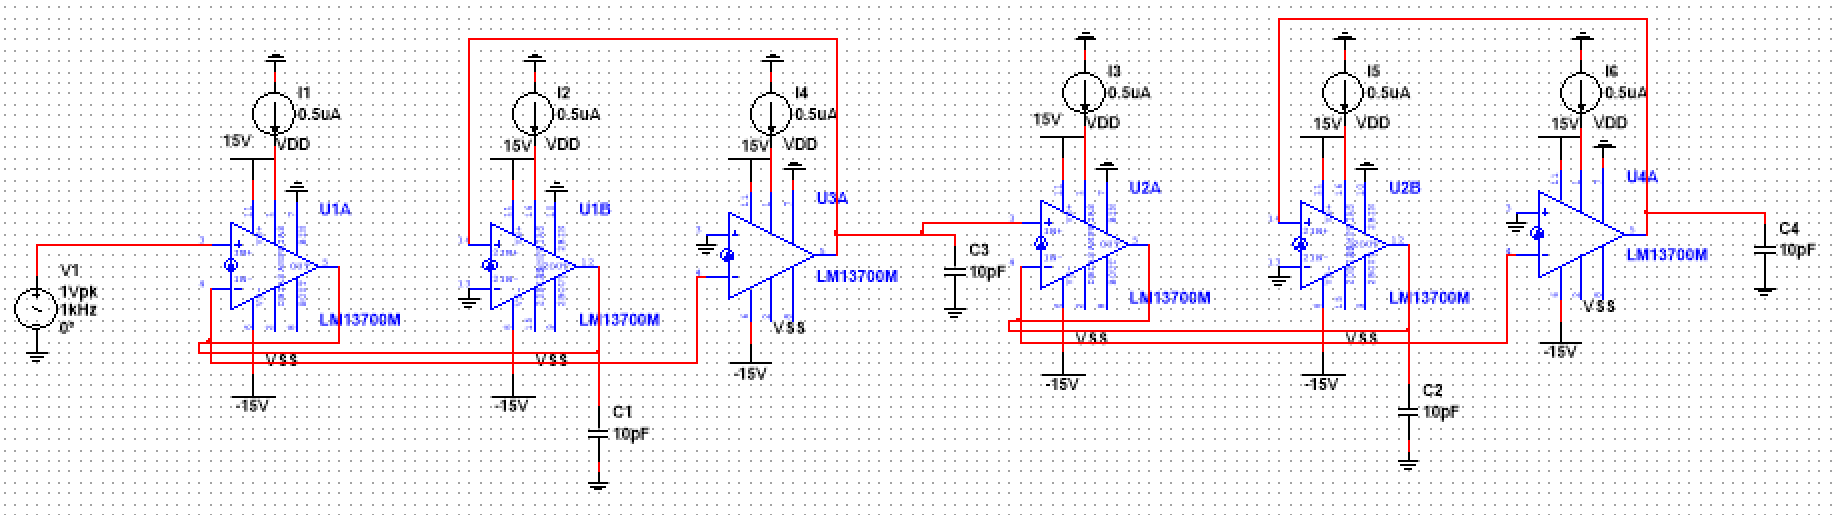
\includegraphics[scale=0.5]{lpbp32.png}
\caption{Schéma zapojení DP 4. řádu}
\end{figure}\begin{figure}[h]
\centering
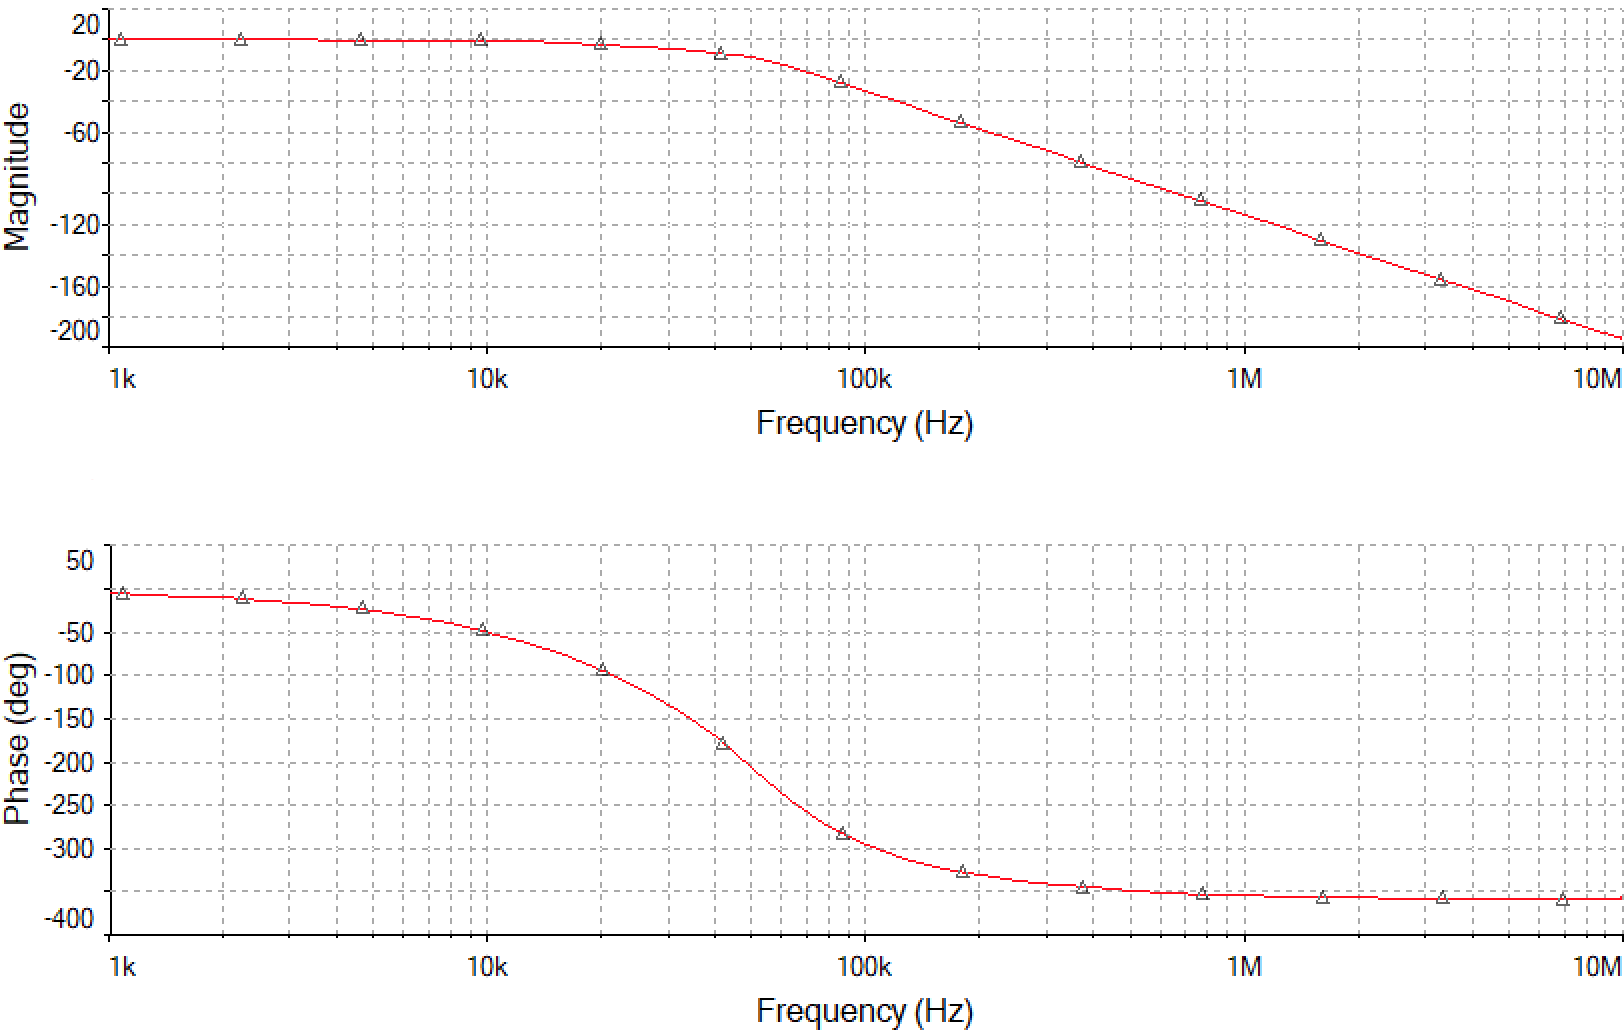
\includegraphics[scale=0.45]{bplp3.png}
\caption{Amplitudová a fázová charakteristika DP 4. řádu}
\end{figure}
\subsection{Pásmová propust 2. řádu}\label{s:PP2}
Horní propust druhého řádu má přenos v nule nulový $H_{0} = 0$. Přenosová funkce je
\begin{align}
H(j\omega) = \frac{H_{\infty} (j\omega) ^2}{(j\omega)^2 + \frac{\omega _c}{Q}(j\omega) + \omega _c ^2}.
\end{align}
\noindent Pásmovou propust lze získat zapojením dolní a horní propusti.
\begin{figure}[h]
\centering
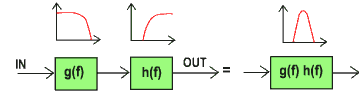
\includegraphics[scale=0.9]{fig9.png}
\caption{Násobení přenosů \cite{13}}
\end{figure}
\noindent Pásmová propust má přenos v nule i nekonečnu nulový $H_{0} = H_{\infty} = 0$. Přenosová funkce je
\begin{align}
H(j\omega) = \frac{H_{B} \frac{\omega _c}{Q} (j\omega) }{(j\omega)^2 + \frac{\omega _c}{Q}(j\omega) + \omega _c ^2}.
\end{align}
\begin{figure}[h]
\centering
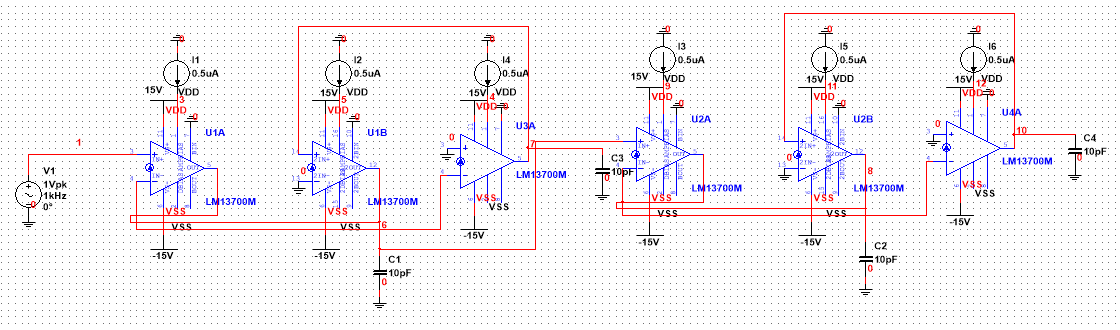
\includegraphics[scale=0.6]{PP2O.png}
\caption{Schéma zapojení PP 2. řádu}
\end{figure}
\begin{figure}[h]
\centering
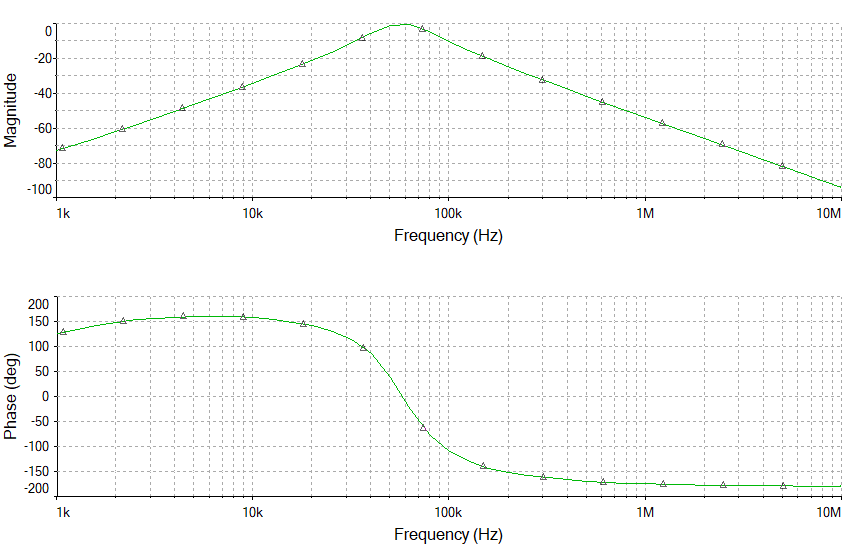
\includegraphics[scale=0.6]{PP2O2.png}
\caption{Amplitudová a fázová charakteristika PP 2. řádu}
\end{figure}
\subsection{Pásmová propust 4. řádu}\label{s:PP4}
\noindent Zapojením dvou PP 2. řádu byla obdržena PP 4.řádu s poklesem -80 dB/dek. 
\begin{figure}[h]
\centering
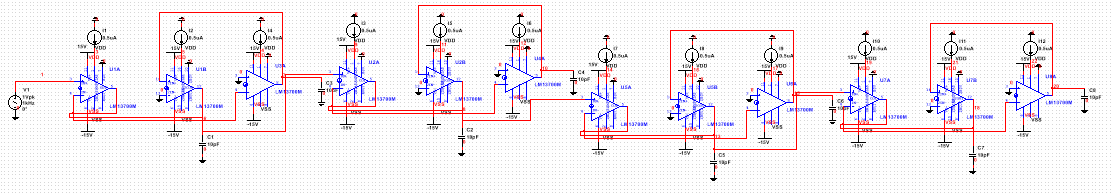
\includegraphics[scale=0.5]{PP4O.png}
\caption{Schéma zapojení PP 4. řádu}
\end{figure}
\begin{figure}[h]
\centering
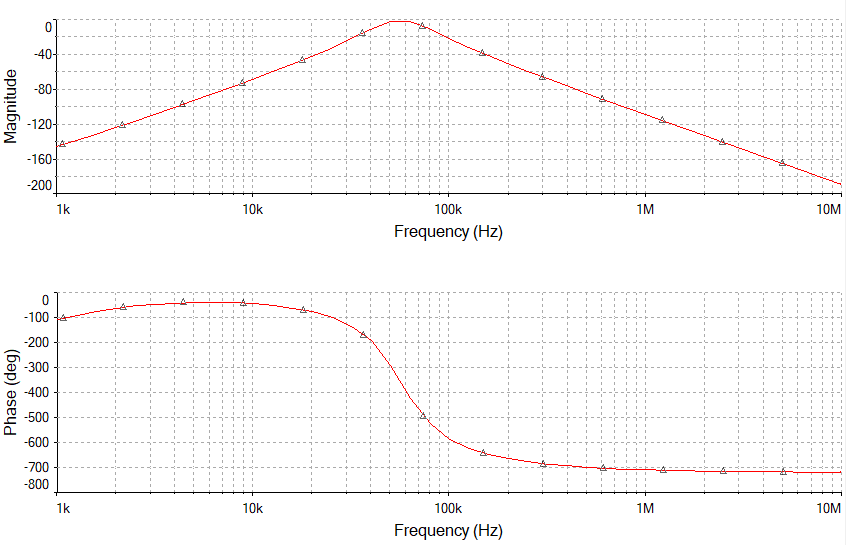
\includegraphics[scale=0.6]{PP4O2.png}
\caption{Amplitudová a fázová charakteristika PP 4. řádu}
\end{figure}